%% LyX 2.4.3 created this file.  For more info, see https://www.lyx.org/.
%% Do not edit unless you really know what you are doing.
\documentclass[11pt,oneside,czech,american]{book}
\usepackage[T1]{fontenc}
\usepackage[utf8]{inputenc}
\setcounter{secnumdepth}{3}
\usepackage{url}
\usepackage{amsmath}
\usepackage{amsthm}
\usepackage{amssymb}
\usepackage{graphicx}
\usepackage{minted}
\usepackage[a4paper]{geometry}
\geometry{verbose,tmargin=4cm,bmargin=3cm,lmargin=3cm,rmargin=2.5cm,headheight=0.8cm,headsep=1cm,footskip=0.5cm}
\pagestyle{headings}
\usepackage{setspace}

\makeatletter
%%%%%%%%%%%%%%%%%%%%%%%%%%%%%% Textclass specific LaTeX commands.
\newenvironment{lyxlist}[1]
	{\begin{list}{}
		{\settowidth{\labelwidth}{#1}
		 \setlength{\leftmargin}{\labelwidth}
		 \addtolength{\leftmargin}{\labelsep}
		 \renewcommand{\makelabel}[1]{##1\hfil}}}
	{\end{list}}

%%%%%%%%%%%%%%%%%%%%%%%%%%%%%% User specified LaTeX commands.
%% Font setup: please leave the LyX font settings all set to 'default'
%% if you want to use any of these packages:

%% Use Times New Roman font for text and Belleek font for math
%% Please make sure that the 'esint' package is turned off in the
%% 'Math options' page.
\usepackage[varg]{txfonts}

%% Use Utopia text with Fourier-GUTenberg math
%\usepackage{fourier}

%% Bitstream Charter text with Math Design math
%\usepackage[charter]{mathdesign}

%%---------------------------------------------------------------------

%% Make the multiline figure/table captions indent so that the second
%% line "hangs" right below the first one.
%\usepackage[format=hang]{caption}

%% Indent even the first paragraph in each section
\usepackage{indentfirst}

%%---------------------------------------------------------------------

\usepackage{pdfpages}

%%---------------------------------------------------------------------

%% Disable page numbers in the TOC. LOF, LOT (TOC automatically
%% adds \thispagestyle{chapter} if not overriden
%\addtocontents{toc}{\protect\thispagestyle{empty}}
%\addtocontents{lof}{\protect\thispagestyle{empty}}
%\addtocontents{lot}{\protect\thispagestyle{empty}}

%% Shifts the top line of the TOC (not the title) 1cm upwards
%% so that the whole TOC fits on 1 page. Additional page size
%% adjustment is performed at the point where the TOC
%% is inserted.
%\addtocontents{toc}{\protect\vspace{-1cm}}

%%---------------------------------------------------------------------

% completely avoid orphans (first lines of a new paragraph on the bottom of a page)
\clubpenalty=9500

% completely avoid widows (last lines of paragraph on a new page)
\widowpenalty=9500

% disable hyphenation of acronyms
\hyphenation{CDFA HARDI HiPPIES IKEM InterTrack MEGIDDO MIMD MPFA DICOM ASCLEPIOS MedInria}

%%---------------------------------------------------------------------

%% Print out all vectors in bold type instead of printing an arrow above them
\renewcommand{\vec}[1]{\boldsymbol{#1}}

% Replace standard \cite by the parenthetical variant \citep
%\renewcommand{\cite}{\citep}

\makeatother
\bibliography{export}
\bibliographystyle{unsrt}
\usepackage{biblatex}
\usepackage{babel}
\usepackage{hyperref}
\begin{document}
\def\documentdate{August 4, 2025}

%%\def\documentdate{\today}

\pagestyle{empty}
{\centering

\noindent{}%
\begin{minipage}[c]{3cm}%
\begin{center}

\includegraphics[width=3cm,keepaspectratio,height=3cm]{Images/TITLE/cvut}
\par\end{center}%
\end{minipage}%
\begin{minipage}[c]{0.6\linewidth}%
\begin{center}
{\large\textsc{Czech Technical University in Prague}}{\large}\\
{\large Faculty of Nuclear Sciences and Physical Engineering}
\par\end{center}%
\end{minipage}%
\begin{minipage}[c]{3cm}%
\begin{center}

\includegraphics[width=3cm,keepaspectratio,height=3cm]{Images/TITLE/fjfi}
\par\end{center}%
\end{minipage}

\vspace{3cm}

{\huge\textbf{Web application for team work organization}}{\huge\par}

\vspace{1cm}

\selectlanguage{czech}%
{\huge\textbf{Webová aplikace pro organizaci týmové práce}}{\huge\par}

\selectlanguage{american}%
\vspace{2cm}

{\large Bachelor's Degree Project}{\large\par}

}

\vfill{}

\begin{lyxlist}{MMMMMMMMM}
\begin{singlespace}
\item [{Author:}] \textbf{Kirill Borodinskiy}
\item [{Supervisor:}] \textbf{doc. Ing. Miroslav Virius, CSc.}
\item [{Academic~year:}] 2024/2025
\end{singlespace}
\end{lyxlist}

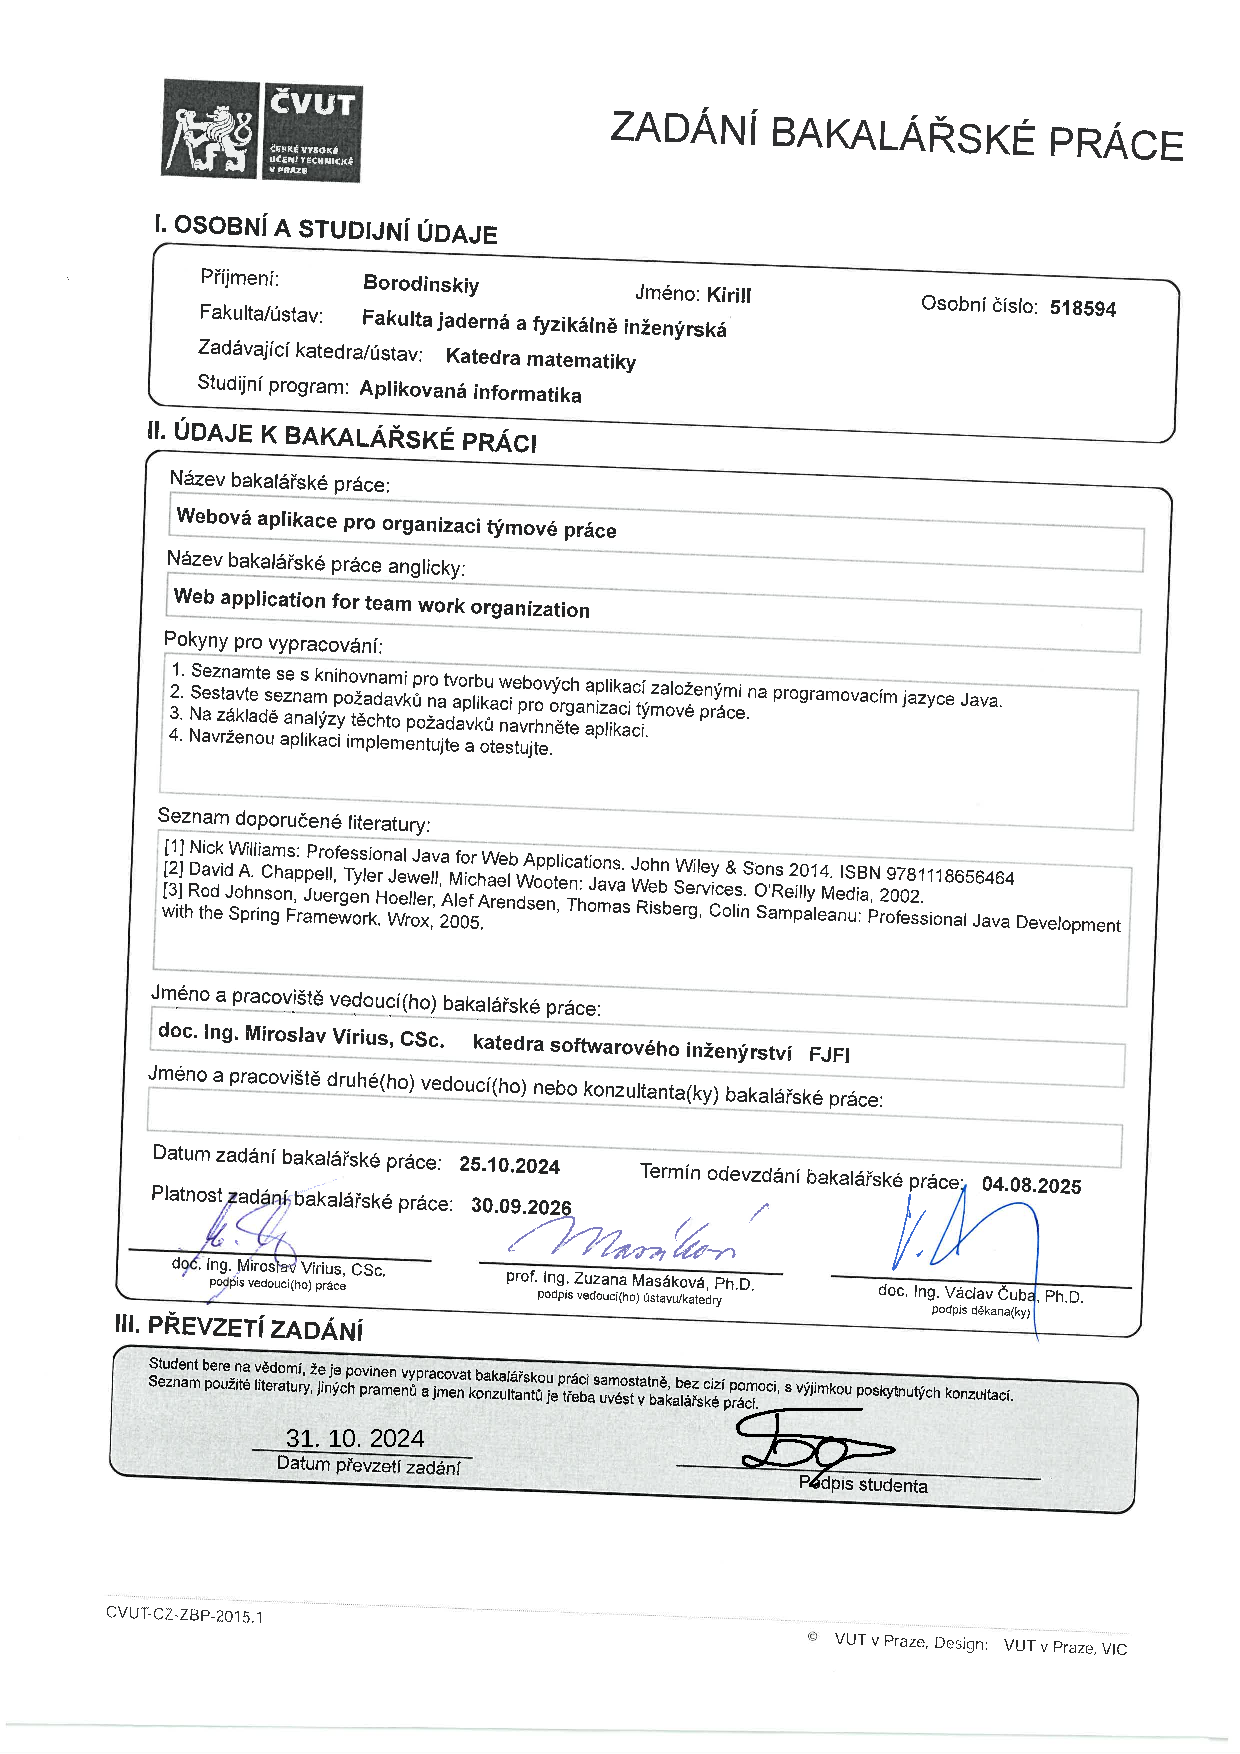
\includepdf[]{BPZADANI.pdf}

\noindent{\Large\emph{Acknowledgment:}}{\Large\par}

\noindent I would like to thank my mother Elena and my girlfriend Anastasiia for their moral support.
I would like to thank my supervisor, Miroslav Virius, for their help in organization of my bachelor's thesis project.

\vfill

\noindent{\Large\emph{Author's declaration:}}{\Large\par}

\noindent I declare that this Bachelor's Degree Project is entirely
my own work and I have listed all the used sources in the bibliography.
AI tools were used in full accordance with the guidelines established
by CTU in Prague.

\bigskip{}

\noindent Prague, \documentdate\hfill{}Kirill Borodinskiy

\vspace{2cm}

\newpage{}

\selectlanguage{czech}%
\begin{onehalfspace}
\noindent\emph{Název práce:}

\noindent\textbf{Webová aplikace pro organizaci týmové práce}
\end{onehalfspace}

\bigskip{}

\noindent\emph{Autor:} Kirill Borodinskiy

\bigskip{}

\noindent\emph{Studijní program:} Celý název studijního programu
(nikoliv zkratka)\bigskip{}

\noindent\emph{Specializace:} Celý název specializace (Pokud se studijní
program nedělí na specializace, tuto řádku odstranit.)

\bigskip{}

\noindent\emph{Druh práce:} Bakalářská práce

\bigskip{}

\noindent\emph{Vedoucí práce:}doc.
Ing.
Miroslav Virius, CSc., DrSc.,
pracoviště školitele (název instituce, fakulty, katedry)

\bigskip{}

\bigskip{}

\noindent\emph{Abstrakt:} Abstrakt max.
na 10 řádků.
Abstrakt max.
na 10 řádků.
Abstrakt max.
na 10 řádků.
Abstrakt max.
na 10 řádků.
Abstrakt max.
na 10 řádků.
Abstrakt max.
na 10 řádků.
Abstrakt max.
na 10 řádků.
Abstrakt max.
na 10 řádků.
Abstrakt max.
na 10 řádků.
Abstrakt max.
na 10 řádků.
Abstrakt max.
na 10 řádků.
Abstrakt max.
na 10 řádků.
Abstrakt max.
na 10 řádků.
Abstrakt max.
na 10 řádků.
Abstrakt max.
na 10 řádků.
Abstrakt max.
na 10 řádků.
Abstrakt max.
na 10 řádků.
Abstrakt max.
na 10 řádků.
Abstrakt max.
na 10 řádků.
Abstrakt max.
na 10 řádků.
Abstrakt max.
na 10 řádků.
Abstrakt max.
na 10 řádků.
Abstrakt max.
na 10 řádků.
Abstrakt max.
na 10 řádků.
Abstrakt max.
na 10 řádků.
Abstrakt max.
na 10 řádků.
Abstrakt max.
na 10 řádků.
Abstrakt max.
na 10 řádků.
Abstrakt max.
na 10 řádků.

\bigskip{}

\noindent\emph{Klíčová slova:} klíčová slova (nebo výrazy) seřazená
podle abecedy a oddělená čárkou

\selectlanguage{american}%
\vfill{}
~

\begin{onehalfspace}
\noindent\emph{Title:}

\noindent\textbf{Title of the Work}
\end{onehalfspace}

\bigskip{}

\noindent\emph{Author:} Kirill Borodinskiy

\bigskip{}

\noindent\emph{Abstract:} Max.
10 lines of English abstract text.
Max.
10 lines of English abstract text.
Max.
10 lines of English abstract
text.
Max.
10 lines of English abstract text.
Max.
10 lines of English
abstract text.
Max.
10 lines of English abstract text.
Max.
10 lines
of English abstract text.
Max.
10 lines of English abstract text.
Max.
10 lines of English abstract text.
Max.
10 lines of English abstract
text.
Max.
10 lines of English abstract text.
Max.
10 lines of English
abstract text.
Max.
10 lines of English abstract text.
Max.
10 lines
of English abstract text.
Max.
10 lines of English abstract text.
Max.
10 lines of English abstract text.
Max.
10 lines of English abstract
text.
Max.
10 lines of English abstract text.
Max.
10 lines of English
abstract text.
Max.
10 lines of English abstract text.
Max.
10 lines
of English abstract text.
Max.
10 lines of English abstract text.
Max.
10 lines of English abstract text.
Max.
10 lines of English abstract
text.
Max.
10 lines of English abstract text.

\bigskip{}

\noindent\emph{Key words:} keywords in alphabetical order separated
by commas

\newpage{}

\pagestyle{plain}

\tableofcontents{}

\newpage{}







\chapter{Introduction}\label{ch:introduction}
\section*{Motivation}
Efficient team schedule planning is a complex challenge, particularly in organizations that require real-time coordination and resource management.
Existing scheduling services often have significant limitations, such as proprietary nature, lack of customization, and dependence on third-party infrastructure.
This project aims to develop a self-hosted open-source booking system designed for organizations that need a private, adaptable scheduling solution.
The system will provide a web-based interface where users can:
\begin{itemize}
    \item Make and manage reservations
    \item Check real-time room availability
    \item  Filter bookings by person or room
    \item View all reservations on a centralized calendar
\end{itemize}

The backend will be built using the Spring Framework, ensuring scalability, security, and ease of integration with existing infrastructure.
Unlike cloud-based alternatives, this system will store all data locally, giving organizations complete privacy and control over scheduling information.
By combining flexibility, transparency, and data privacy, this project can provide a practical alternative to commercial scheduling tools, empowering organizations with greater autonomy and customization options.
\addcontentsline{toc}{section}{Motivation}


\pagestyle{headings}
Here we will talk about why the calendar is needed

Firstly, lets take a look at the current solution used by my university,CTU. Rozvrh.fjfi.cvut.cz is a website where students can see their schedule.
\section{The current solution}\label{sec:the-current-solution}
\begin{figure}[h]
  \centering
  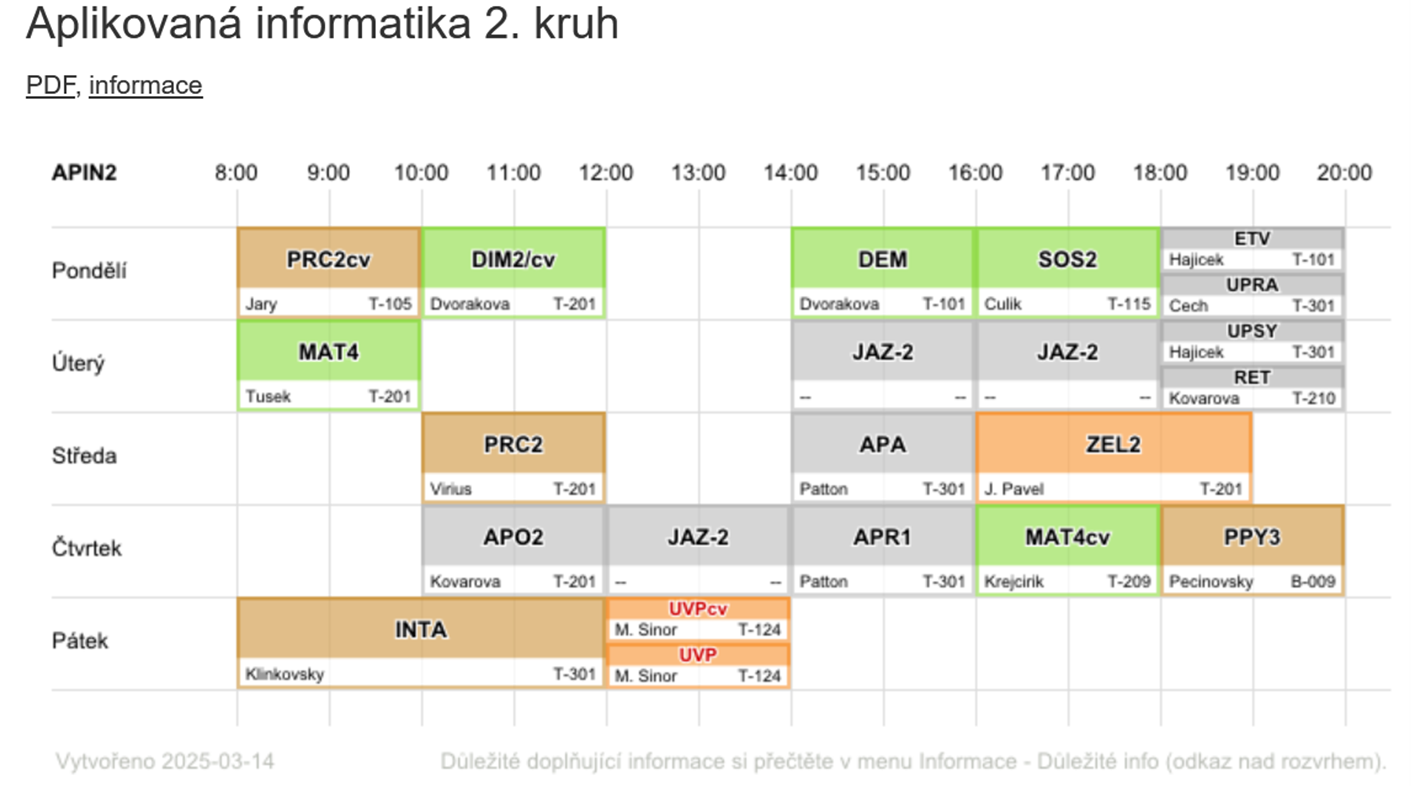
\includegraphics[width=0.6\textwidth]{img}
  \caption{Screenshot of the current solution}
  \label{fig:rozvrh}
\end{figure}

It can be seen on~\ref{fig:rozvrh} that while the website completes its main purpose, it is not customizable, which makes it hard to use.
For example, if a student has a class that is from another year or/and program, they have to look at another picture and manually compare them.
From my experience, many students have screenshots on their phones and they cross-out the classes that they are not registered to.
They may have a few screenshots, for different programs or years.
It is not a good solution, as it allows for misunderstandings and mistakes.

This is why a project focused on creating a calendar that is easy to use and customizable is needed.
\section{The solution}\label{sec:the-solution}
\begin{figure}[h]
  \centering
  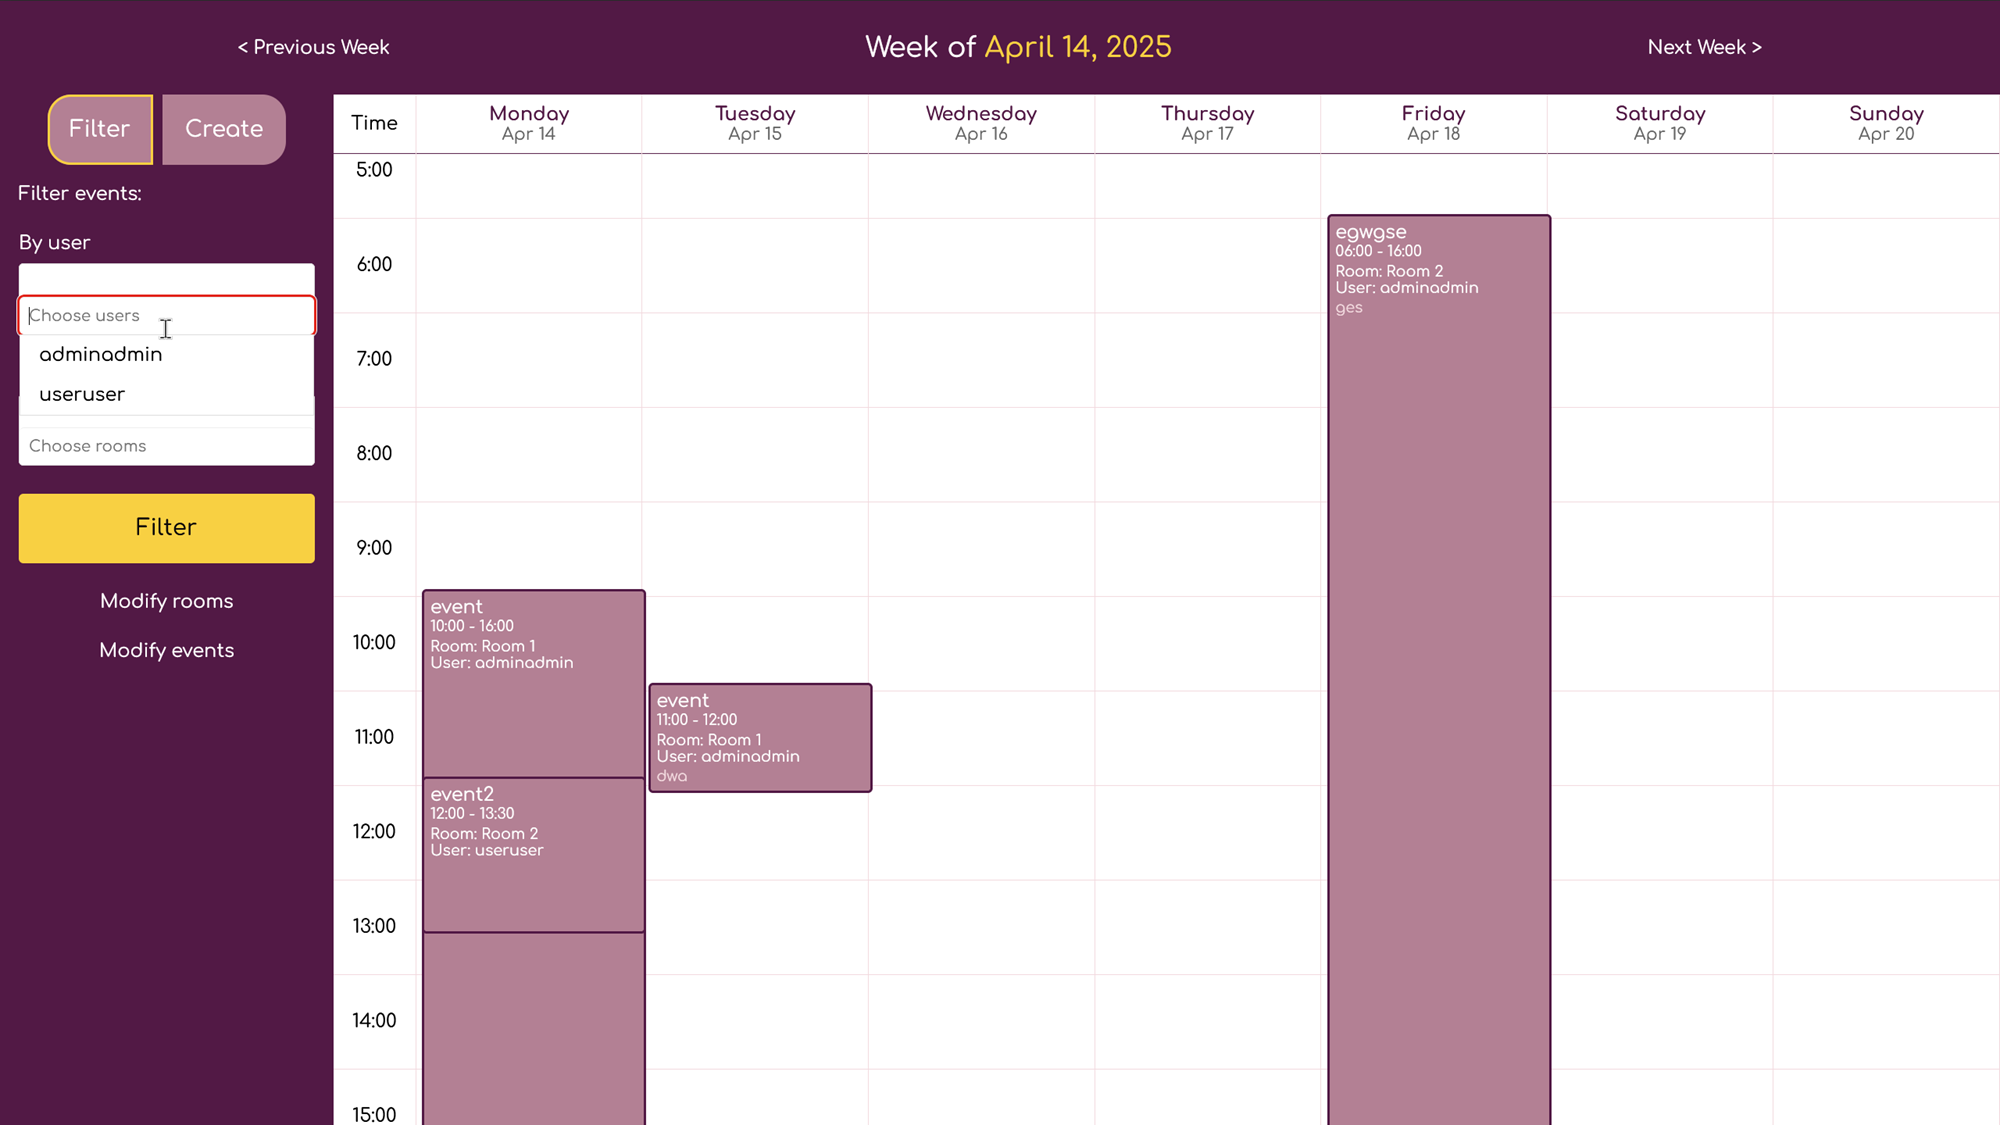
\includegraphics[width=0.6\textwidth]{TeamJob}
  \caption{Screenshot of the new solution}
  \label{fig:TeamJob}
\end{figure}
TeamJob is a web application that allows users to filter exactly what they want to see.
By default, all the events that are happening this week are shown.
The user can filter the events by the room and the person that is assigned to this event.
This allows for a more precise view of the calendar, where the user can see only the events that are important to them.
The user can also move between weeks.
A specific day-view allows the user to see the events that are happening on a specific day, if there are too many events to show them all at once.



\chapter{Tools}\label{ch:tools}
\section{Tool Selection and Technology Stack}\label{sec:tools}

This chapter examines the decision-making process behind selecting the technologies and tools for the team-work organization system.
The selection criteria were based on several key factors: project requirements, scalability needs, security considerations, and long-term maintainability.

\subsection{Framework Selection}\label{subsec:framework-selection}

Given the project's requirement to develop a Java application, the framework selection was focused on Java-based solutions.
The primary options considered were \textit{The Spring Framework}, \textit{Spring Boot},  \textit{Jakarta EE} (formerly Java EE), and \textit{Micronaut}.
Although all of these frameworks are capable of building robust web applications, they differ significantly in their approach and complexity.

\textbf{Jakarta EE}, the enterprise edition of Java, provides a comprehensive set of specifications to build enterprise applications.
However, it requires significant boilerplate code and configuration, making it less suitable for this project.
\textbf{Micronaut}, while promising with its ahead-of-time compilation and low memory footprint, is relatively new and has a smaller community compared to Spring Boot.

\textbf{The Spring Framework}, the foundation of Spring Boot, is a comprehensive programming and configuration model for modern Java-based enterprise applications.
It provides a wide range of features including dependency injection, aspect-oriented programming, and transaction management.
However, the Spring Framework requires extensive configuration and setup, which can be time consuming and complex.

\textbf{Spring Boot}, built on top of the Spring Framework, was selected as it addresses these configuration challenges while maintaining all the benefits of the Spring Framework.
It provides the following:
\begin{itemize}
    \item Auto-configuration of Spring Framework components
    \item Embedded servers for simplified deployment
    \item Production-ready features like metrics and health checks
    \item Reduced boilerplate code and configuration
\end{itemize}

This combination of Spring Framework's robust features and Spring Boot's simplified development approach makes it ideal for this project.
The framework's extensive documentation, large community support, and proven track record in enterprise applications further reinforce this choice.

\subsection{Frontend Technology Selection}\label{subsec:frontend-selection}

The selection of front-end technology required careful consideration of integration capabilities with Spring Boot.
\textbf{Thymeleaf}, as a server-side template rendering engine, was identified as the preferred option due to several factors.
It utilizes server-side page rendering to decrease the computational load on client systems.
Its integration of Java with HTML makes it relatively straightforward to use.
Furthermore, it is frequently used in conjunction with the Spring Boot.
Although modern alternatives like \textbf{React} and other JavaScript frameworks are prevalent, they would require significant additional research and development time.

The decision to use Thymeleaf was influenced by the simplicity of combining HTML and Java code in a single file.
However, modern web development requirements necessitated the incorporation of some JavaScript for specific client-side tasks, particularly for handling asynchronous requests and dynamic content updates.

\subsection{Database Selection}\label{subsec:database-selection}

\textbf{PostgreSQL} was selected as the primary database system after evaluating various database options, including NoSQL alternatives.
This choice was driven by PostgreSQL's prevalence in the market and its robust ACID compliance, which ensures data integrity and reliability.
The ACID properties provide essential guarantees for data management:

\begin{itemize}
    \item \textbf{Atomicity}: Ensures transactions are completed entirely or not at all.
    \item \textbf{Consistency}: Maintains database validity through all transactions.
    \item \textbf{Isolation}: Prevents concurrent transactions from interfering with each other.
    \item \textbf{Durability}: Guarantees committed transactions remain permanent.
\end{itemize}

These properties are crucial for maintaining data integrity in a multi-user environment where concurrent access and modifications are common.

\subsection{Security Architecture Decisions}\label{subsec:security-decisions}

The security implementation strategy was developed after careful analysis of the security requirements of modern web applications.
The decision to use \textbf{JWT-based authentication} was made after considering several factors, including the benefits of a stateless architecture that eliminates server-side session storage and improves scalability.
The approach also offers excellent cross-platform compatibility, enabling seamless integration with various clients while maintaining compliance with industry best practices for web security.
Alternative approaches like \textbf{session-based authentication} were evaluated but rejected due to their increased complexity with server-side session storage, increased server resource requirements, and complex session management.


The main security framework used is \textbf{Spring Security}, which provides a comprehensive security solution for Spring-based applications.
Although it is a powerful framework, it is not without its own challenges, such as the need to configure multiple security components and the potential for increased complexity in the codebase.
Still, the benefits of using a well-established security framework benefits the project in the long run.

\subsection{Development Tool Selection}\label{subsec:tool-selection}

The choice of development tools was guided by the need to improve code quality and development efficiency.
\textbf{Lombok} was selected because it effectively reduces boilerplate code without runtime overhead, integrates seamlessly with existing IDEs, and maintains code readability while reducing verbosity.
The IDE used is \textbf{IntelliJ IDEA}, which has excellent support for Java.

\subsection{Containerization Strategy}\label{subsec:containerization}

Containerization was implemented using \textbf{Docker} to ensure consistent deployment across different environments and simplify the development workflow.
The containerization strategy employs a multi-stage build process that optimizes both build time and final image size.
The build process utilizes \textbf{Amazon Corretto JDK 21} to compile the application and run it in a separate dockerfile stage.
The system includes integrated health checks to monitor container status, ensuring reliable operation and quick detection of potential problems.

This containerization approach delivers significant benefits to the project.
It ensures a consistent runtime environment across development, testing, and production stages, eliminating environment-specific issues.
The deployment process is simplified, reducing the complexity of moving the application between different environments.
Container isolation provides an additional layer of security, while the standardized container format enables easy scalability and orchestration capabilities.
Furthermore, this approach effectively eliminates the common ``works on my machine'' problem, as all environments run the same containerized application.
The basics of this approach were learned from the video resource~\cite{LearnDocker}.

\subsection{Technology Stack Integration}\label{subsec:integration}

The selected technologies were tested for their ability to work together.
The integration strategy focused on ensuring compatibility between all components, maintaining optimal system performance across all layers, and creating a system that can be easily updated and modified.
This careful selection and integration of technologies has resulted in a robust, scalable, and maintainable system that meets project requirements while providing a solid foundation for future enhancements.


\chapter{Methods}\label{ch:methods}
This section will focus on the tools and techniques used to create a web application tShreyashVardhan2024o manage time and space resources of an organization.


\section{Defining the toolbelt}\label{sec:defining-the-toolbelt}
% Расписать все варианты и в итоге выбрать итоговый.
% Расписать всю структуру будущюю.
% Интересные инструменты использованные указать.
% Указать алгортм использованный в приложении.
% Реальные человеческие отзывы сделать.

% Spring Boot vs. Spring vs. C# vs. Django vs. Flask
For the programming language, the options were as follows: Java Spring Boot framework, C\#.NET, and Python's Django and Flask.
C\# was first removed, as learning about it would take a considerable amount of time.
Python's Flask is easy to use, but not customizable enough.
Subsequent analysis, as presented in the study~\cite{ShreyashVardhan2024}, indicates that Spring Boot exhibits superior performance.
Moreover, my familiarity with Java might reduce the time required for development.
Consequently, Spring Boot is selected as the back-end framework.
Spring Boot, which is constructed on the Spring Framework, is recognized as a leading framework within the Java ecosystem due to its widespread popularity.
It streamlines the original Spring Framework, thereby facilitating more straightforward maintenance and expediting deployment procedures.
Henceforth, to maintain clarity, the term Spring Boot shall be used exclusively in reference to both the Spring Framework and Spring Boot.

% Google Web Toolkit vs. Thymeleaf vs. React/other JS
An often-utilized integration of back-end and front-end frameworks with Spring Boot is accomplished through Thymeleaf, a template rendering engine which processes page rendering on the server side, thereby reducing computational demand on the client-side systems.
However, alternative solutions are available, including the currently prevalent React framework along with other JavaScript frameworks.
Opting for these alternatives requires considerable investment in research.
Given my proficiency in HTML, the Thymeleaf template system presents a straightforward learning curve.
Nevertheless, a certain degree of JavaScript is essential for contemporary websites, thereby necessitating its use for handling specific tasks such as requests.


% PostgreSQL vs. NoSQL vs. others
For our database, PostgreSQL was chosen, as it is a popular ACID-compliant database.
ACID stands for:
\begin{itemize}
    \item \textbf{Atomicity}: Transaction is either fully completed, or not, with no in-betweens.
    \item \textbf{Consistency}: Guarantees that a transaction brings the database from a valid state to a valid state.
    \item \textbf{Isolation}: Concurrent transactions do not interfere with each other.
    \item \textbf{Durability}: Once a transaction is committed, it stays committed.
\end{itemize}


\subsection{Useful tools}\label{subsec:useful-tools}
In this application, \textit{Lombok} was used to reduce the amount of boilerplate code.
It allows for the usage of annotations such as \texttt{@Getter,@Setter} to automatically generate setters and setters for all fields that need them.
In addition, annotations \texttt{@AllArgsConstructor,@NoArgsConstructor} can automatically create the correct construction function for the class.
Finally, \texttt{@Data} combines \texttt{@Getter,@Setter} and some more functions in one annotation, so the classes remain clean and functional.

The use of the tool is demonstrated in the list~\ref{lst:room-class}.
It can be seen that no setter or getter functions are needed, no construction function is needed, and the class looks clean and complete.


\begin{listing}[H]
    \begin{minted}{java}

@Data
@Entity
@Table(name = "rooms")
@EqualsAndHashCode(callSuper = true)
public class Room extends Auditable {
    @Id
    @GeneratedValue(strategy = GenerationType.IDENTITY)
    private Long id;

    @Column(nullable = false, unique = true)
    private String name;

    @Column()
    private String description;

    @Type(io.hypersistence.utils.hibernate.type.array.ListArrayType.class)
    @Column(name = "tags", columnDefinition = "text[]")
    private Set<String> tags = new HashSet<>();

}
    \end{minted}
    \caption{Lombok-annotated JPA entity}
    \label{lst:room-class}
\end{listing}

\section{Introduction to Spring Boot}\label{sec:introduction-to-spring-boot}

Spring Boot is a tool that allows the programmer to create a web server that uses the Model-View-Controller pattern, MVC for short.

The model is a part responsible for the data logic.
The connection to the database, the processing of the requested data and other back-end transactions are what this part consists of.

The view is a part that displays the data to a user or gathers them from them.
Whether HTML, plain text, or any other format such as our Thymeleaf.

The controller is a connector between the previous two, where the data is additionally processed before being sent into either the database or a client of a user.


\section{Schema of the database}\label{sec:schema-of-the-database}
\begin{figure}[h]
  \centering
  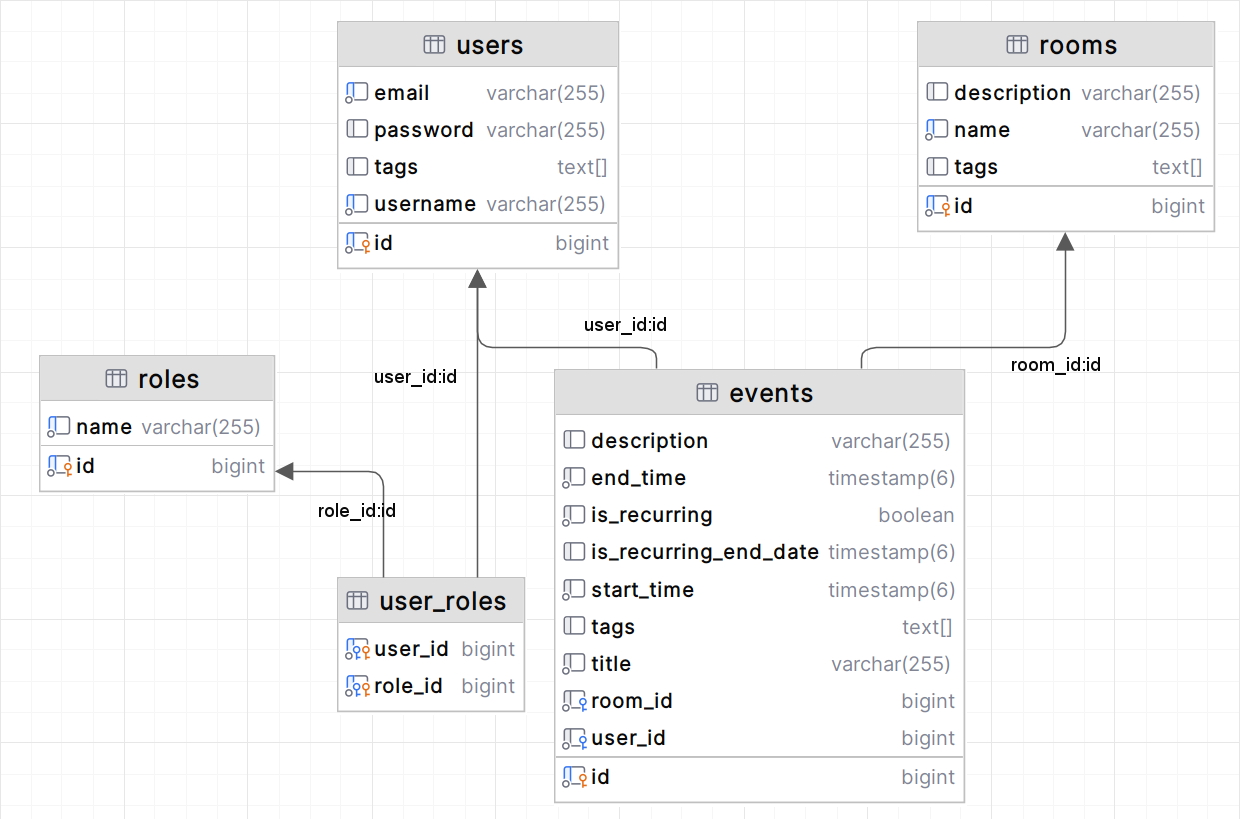
\includegraphics[width=0.6\textwidth]{schemaDB}
  \caption{Schema of the database for the application}
  \label{fig:schemaDB}
\end{figure}

\subsection*{Database \ref{fig:schemaDB} Architecture}

\begin{itemize}
  \item \textbf{users}: Stores user credentials and personal data.
  Each user has a unique \texttt{ID}.

  \item \textbf{roles} \& \textbf{user\_roles}: Implements role-based access control via a many-to-many relation between users and roles.

  \item \textbf{rooms}: Contains information on event locations.
  Each room has a \texttt{name}, \texttt{description} and a unique \texttt{ID}.

  \item \textbf{events}: Represents scheduled activities.
  Includes data such as  \texttt{is\_recurring}, \texttt{title}, \texttt{start\_time} and \texttt{end\_time}.
  Each event references a \texttt{user} and a \texttt{room} that were assigned to this event.

  \item \textbf{users, events }and \textbf{rooms} all contain \texttt{tags} to help categorize them.
\end{itemize}


\newpage%                    NEW PAGE HERE !!!!!!!!!!!!!!!!!!!!!!!!!!!!!!!!!!!!!!!!!!!

\section{The implementation of a Spring Boot application}\label{sec:the-implementation-of-a-spring-boot-application}
In our application, the main controller is CalendarController.
It renders the main page /calendar.
The non-required parameters of a request are: ``\textit{date}'', ``\textit{roomIds}'' and ``\textit{userIds}''.

Parameter \("\)\textit{date}\("\) is simply the day of the week the calendar renders.
If not provided, we use the default value of a current day.

Parameters ``\textit{roomIds}'' and ``\textit{userIds}'' are used to filter out which events the user wants to see in their calendar.
If not provided, events from every room and every user are displayed.

In this controller a week around the current day is generated, all the events that are happening in that week are found and are put into an array that is then sent with the model.




\newpage%                    NEW PAGE HERE !!!!!!!!!!!!!!!!!!!!!!!!!!!!!!!!!!!!!!!!!!!

\subsection{The architecture of the application}\label{subsec:the-architecture-of-the-application}

The main file responsible for most tasks is CalendarController, where the \texttt{/calendar} endpoint is located.

The \texttt{/calendar} takes 3 non-required parameters.
\begin{itemize}
    \item \textbf{date}: Show the events that happen on the week of the day sent.
    \item \textbf{userIds}: Filter the users shown on the central calendar.
    \item \textbf{roomIds}: Filter rooms displayed in the central calendar.
\end{itemize}
Then, the \texttt{EventRepository} is used to find all the events that are happening in the week of the date sent.
The \texttt{EventRepository} is a Spring Data JPA repository that allows for easy access to the database.
They are split into a list of events that are happening on a specific day, where the days are filtered by comparing the \texttt{userIds} and \texttt{roomIds} with the events that are in the database.
the data inside each event is such:
\begin{itemize}
    \item \textbf{eventId}
    \item \textbf{eventTitle}
    \item \textbf{eventDescription}
    \item \textbf{eventStartTime} - the time when the event starts in LocalDateTime format.
    \item \textbf{eventEndTime}
    \item \textbf{eventRoomId} - the room that is assigned to this event.
    \item \textbf{eventUserId} - the user that is assigned to this event.
    \item \textbf{eventTags} - the tags that are assigned to this event.
    \item \textbf{eventIsRecurring} - if the event is recurring or not.
\end{itemize}
The \texttt{/calendar} then sends such data to \texttt{calendar.html}:
\begin{itemize}
    \item \textbf{userIds} \& \textbf{roomIds} (if supplied from request).
    \item \textbf{selectedDate} (if not provided, current date is used).
    \item \textbf{nextWeek} \& \textbf{previousWeek} to enable navigation within weeks.
    \item \textbf{currentWeekStart}.
    \item \textbf{weekDays} - a list of events that take place on a specific day.
    \item \textbf{eventRepository}, \textbf{userRepository} and \textbf{roomRepository}
\end{itemize}

\subsection{Additional Calendar Endpoints}\label{subsec:additional-calendar-endpoints}

The CalendarController also provides a day view endpoint at \texttt{/calendar/day}, which displays events for a specific day organized by room.
This endpoint accepts the following parameters:

\begin{itemize}
    \item \textbf{date} (required): The specific date to display events for.
    \item \textbf{userIds} (optional): Filter events by specific users.
    \item \textbf{roomIds} (optional): Filter events by specific rooms.
\end{itemize}

The day view provides a more detailed perspective of events occurring on a single day, organized by room.
This is particularly useful when there are many events scheduled on a specific day, making the weekly view potentially cluttered.

Another important endpoint is \texttt{/calendar/findAvailable}, which allows users to search for available resources (rooms, users, or events) based on various criteria:

\begin{itemize}
    \item \textbf{searchType}: Specifies whether to search for ``rooms'', ``users'', or ``events''.
    \item \textbf{tags}: Allows filtering by specific tags associated with the resources.
    \item \textbf{date}: The date to search for availability (defaults to current date if not provided).
    \item \textbf{startTime} \& \textbf{endTime}: The time range to check for availability.
\end{itemize}

This functionality is particularly valuable for quickly identifying available resources during a specific time slot, facilitating efficient scheduling and resource allocation.

\subsection{The findAvailable Algorithm}\label{subsec:findavailable-algorithm}

The findAvailable algorithm is a sophisticated process that identifies available time slots for rooms, users, or events within a specified time range.
Here's how it works:

\begin{enumerate}
    \item \textbf{Input Processing}: The algorithm accepts several parameters:
    \begin{itemize}
        \item \texttt{searchType}: Determines whether to search for available rooms, users, or events (By default, ``rooms'')
        \item \texttt{tags}: Optional tags to filter resources by (e.g., ``projector'', ``whiteboard'', etc.)
        \item \texttt{date}, \texttt{startTime}, \texttt{endTime}: Define the time range to check (defaulting to the current date if not provided)
        \item \texttt{durationMinutes}: Minimum duration required for an available time slot (By default, 30 minutes)
    \end{itemize}

    \item \textbf{Data Collection}: The system retrieves all events that overlap with the specified time range.

    \item \textbf{Entity Filtering}: Based on the searchType, the algorithm filters entities (rooms, users, or events) by the provided tags.

    \item \textbf{Availability Calculation}: For each entity, the algorithm:
    \begin{itemize}
        \item Identifies all events associated with the entity
        \item Creates a list of occupied time slots from these events
        \item Sorts occupied slots by start time and merges any overlapping slots
        \item Calculates unoccupied time slots by finding gaps between occupied slots
        \item Filters unoccupied slots by the minimum duration requirement
    \end{itemize}

    \item \textbf{Result Generation}: The algorithm creates a list of available entities along with their unoccupied time slots.
\end{enumerate}

\subsubsection{Implementation Details}

The key component of this algorithm is the \texttt{calculateUnoccupiedTimesFromOccupied} method, which efficiently identifies available time slots by:

\begin{enumerate}
    \item Sorting occupied time slots by start time
    \item Merging overlapping occupied slots
    \item Iterating through occupied slots to find gaps (unoccupied times)
    \item Filtering unoccupied slots by minimum duration
    \item Sorting the resulting unoccupied slots
\end{enumerate}

\subsubsection{Handling Overlapping Time Slots}

A critical aspect of the algorithm is the \texttt{removeOverlaps} method, which merges overlapping time intervals:

\begin{enumerate}
    \item The method requires that time slots are already sorted by start time
    \item It iterates through adjacent pairs of time slots
    \item When two slots overlap (the end time of one is after the start time of the next), they are merged
    \item The merged slot spans from the start time of the first slot to the end time of the second slot
    \item The second slot is removed from the list, and the iteration index is decremented to recheck the newly merged slot
    \item This process continues until no more overlaps exist
\end{enumerate}

\subsubsection{Calculating Unoccupied Time Slots}

The algorithm identifies unoccupied time slots through the following process:

\begin{enumerate}
    \item Start with the requested start time as the current point
    \item For each occupied time slot (after sorting and merging):
        \begin{itemize}
            \item If the current point is before the start of the occupied slot, add an unoccupied slot from the current point to the start of the occupied slot
            \item Update the current point to the end of the occupied slot
        \end{itemize}
    \item After processing all occupied slots, if the current point is before the requested end time, add a final unoccupied slot from the current point to the requested end time
    \item Filter the resulting unoccupied slots to include only those that meet or exceed the minimum duration requirement
\end{enumerate}

\subsubsection{Edge Case Handling}

The algorithm handles several edge cases:

\begin{itemize}
    \item \textbf{Empty tag sets}: If no tags are specified, all entities of the requested type are included
    \item \textbf{No events}: If there are no events in the specified time range, the entire range is considered unoccupied
    \item \textbf{Completely occupied time range}: If the entire time range is occupied, no unoccupied slots are returned
    \item \textbf{Invalid entity type}: If an invalid entity type is provided, an IllegalArgumentException is thrown
\end{itemize}

\subsubsection{Performance Considerations}

Several optimizations enhance the algorithm's performance:

\begin{itemize}
    \item \textbf{Early filtering}: Events are filtered by time range at the database level before further processing
    \item \textbf{Efficient tag filtering}: Uses \texttt{Collections.disjoint()} to quickly check for tag matches
    \item \textbf{Sorting before processing}: Ensures that time slot operations can be performed in a single pass
    \item \textbf{Stream operations}: Leverages Java streams for concise and efficient filtering operations
\end{itemize}

This approach ensures that users can quickly find available resources that meet their specific time and duration requirements, optimizing resource allocation and scheduling efficiency.
The algorithm's modular design also allows for easy extension to support additional entity types in the future.

\section{Authentication and Security}\label{sec:authentication-and-security}

The application implements a robust security system using JSON Web Tokens (JWT) for authentication.
The SecurityController handles the authentication process through several REST endpoints:

\begin{itemize}
    \item \texttt{/auth/signin} (POST): Authenticates a user with username and password, generating a JWT token stored in a secure HTTP-only cookie.
    \item \texttt{/auth/signup} (POST): Registers a new user with username, email, and password.
    The password is securely hashed before storage.
    \item \texttt{/auth/signout} (POST): Logs out a user by invalidating their JWT cookie.
\end{itemize}

The JWT implementation enhances security by:
\begin{itemize}
    \item Using HTTP-only cookies to prevent JavaScript access to the token
    \item Setting the Secure flag to ensure transmission only over HTTPS
    \item Implementing token expiration to limit the window of vulnerability
\end{itemize}

The MainController provides view endpoints for authentication-related pages:
\begin{itemize}
    \item \texttt{/}, \texttt{/login}, \texttt{/signin}: All route to the sign-in page
    \item \texttt{/register}, \texttt{/signup}: Route to the registration page
    \item \texttt{/signout}: Routes to the sign-out page
\end{itemize}

\section{Configuration and Administration}\label{sec:configuration-and-administration}

The application provides both view-based and REST API endpoints for configuration and administration.

The ConfigController offers view endpoints for managing system entities:
\begin{itemize}
    \item \texttt{/config/rooms}: Lists all rooms in the system
    \item \texttt{/config/events}: Lists all events in the system
    \item \texttt{/config/users}: Lists all users in the system
\end{itemize}

For programmatic interaction, the RestConfigController provides REST API endpoints:
\begin{itemize}
    \item \texttt{/api/v1/addrooms} (POST): Creates a new room
    \item \texttt{/api/v1/addevents} (POST): Creates a new event, with conflict checking
    \item \texttt{/api/v1/checkavailability} (POST): Verifies if a room is available during a specific time period
    \item \texttt{/api/v1/deleterooms/\{id\}} (DELETE): Removes a room by ID
    \item \texttt{/api/v1/deleteevents/\{id\}} (DELETE): Removes an event by ID
    \item \texttt{/api/v1/validateJWT} (POST): Validates the current JWT token
\end{itemize}

\section{Error Handling}\label{sec:error-handling}

The application implements a CustomErrorController that provides a unified approach to error handling.
When an error occurs, the controller captures details such as:
\begin{itemize}
    \item Error status code
    \item Exception type
    \item Error message
    \item Request path that caused the error
    \item Stack trace (in development environments)
\end{itemize}

This information is then rendered in a user-friendly error page, enhancing the debugging process while maintaining a consistent user experience even when errors occur.
This could be further improved by adding a system that would notify the administrator about the error, ensuring that it is addressed promptly.


\chapter*{Conclusion}

\pagestyle{plain}

\addcontentsline{toc}{chapter}{Conclusion}

Text of the conclusion\ldots{}
\begin{thebibliography}{1}
\bibitem{Allen-Cahn}S. Allen, J. W. Cahn: \emph{A microscopic theory
for antiphase boundary motion and its application to antiphase domain
coarsening}.
Acta Metall., 27:1084-1095, 1979.

\bibitem{CINECA}G. Ballabio et al.: \emph{High Performance Systems
User Guide}.
High Performance Systems Department, CINECA, Bologna,
2005. \url{www.cineca.it}

\bibitem{rumpf3}J. Becker, T. Preusser, M. Rumpf: \emph{PDE methods
in flow simulation post processing}.
Computing and Visualization in
Science, 3(3):159-167, 2000.

\end{thebibliography}

\end{document}
